\documentclass[unicode,11pt,a4paper,oneside,numbers=endperiod,openany]{scrartcl}

\usepackage{ifthen}
\usepackage[utf8]{inputenc}
\usepackage{graphics}
\usepackage{graphicx}
\usepackage{hyperref}

\pagestyle{plain}
\voffset -5mm
\oddsidemargin  0mm
\evensidemargin -11mm
\marginparwidth 2cm
\marginparsep 0pt
\topmargin 0mm
\headheight 0pt
\headsep 0pt
\topskip 0pt        
\textheight 255mm
\textwidth 165mm

\newcommand{\duedate} {}
\newcommand{\setduedate}[1]{%
\renewcommand\duedate {Due date:~ #1}}
\newcommand\isassignment {false}
\newcommand{\setassignment}{\renewcommand\isassignment {true}}
\newcommand{\ifassignment}[1]{\ifthenelse{\boolean{\isassignment}}{#1}{}}
\newcommand{\ifnotassignment}[1]{\ifthenelse{\boolean{\isassignment}}{}{#1}}

\newcommand{\assignmentpolicy}{
\begin{table}[h]
\begin{center}
\scalebox{0.8} {%
\begin{tabular}{|p{0.02cm}p{16cm}|}
\hline
&\\
\multicolumn{2}{|c|}{\Large\textbf{HPC Lab for CSE 2024 ---  Submission Instructions}}\\
\multicolumn{2}{|c|}{\large\textbf{(Please, notice that following instructions are mandatory: }}\\
\multicolumn{2}{|c|}{\large\textbf{submissions that don't comply with, won't be considered)}}\\
&\\
\textbullet & Assignments must be submitted to \href{https://moodle-app2.let.ethz.ch/course/view.php?id=22516}{Moodle} (i.e. in electronic format).\\
\textbullet & Provide both executable package and sources (e.g. C/C++ files, Matlab). 
If you are using libraries, please add them in the file. Sources must be organized in directories called:\\
\multicolumn{2}{|c|}{\textit{Project\_number\_lastname\_firstname}}\\
& and  the  file must be called:\\
\multicolumn{2}{|c|}{\textit{project\_number\_lastname\_firstname.zip}}\\
\multicolumn{2}{|c|}{\textit{project\_number\_lastname\_firstname.pdf}}\\
\textbullet &  The TAs will grade your project by reviewing your project write-up, and looking at the implementation 
                 you attempted, and benchmarking your code's performance.\\

\textbullet & You are allowed to discuss all questions with anyone you like; however: (i) your submission must list anyone you discussed problems with and (ii) you must write up your submission independently.\\
\hline
\end{tabular}
}
\end{center}
\end{table}
}
\newcommand{\punkte}[1]{\hspace{1ex}\emph{\mdseries\hfill(#1~\ifcase#1{Points}\or{Points}\else{Points}\fi)}}


\newcommand\serieheader[6]{
\thispagestyle{empty}%
\begin{flushleft}

\includegraphics[width=0.4\textwidth]{ETHlogo_13}
\end{flushleft}
  \noindent%
  {\large\ignorespaces{\textbf{#1}}\hspace{\fill}\ignorespaces{ \textbf{#2}}}\\ \\%
  {\large\ignorespaces #3 \hspace{\fill}\ignorespaces #4}\\
  \noindent%
  \bigskip
  \hrule\par\bigskip\noindent%
  \bigskip {\ignorespaces {\Large{\textbf{#5}}}
  \hspace{\fill}\ignorespaces \large \ifthenelse{\boolean{\isassignment}}{\duedate}{#6}}
  \hrule\par\bigskip\noindent%  \linebreak
 }

\makeatletter
\def\enumerateMod{\ifnum \@enumdepth >3 \@toodeep\else
      \advance\@enumdepth \@ne
      \edef\@enumctr{enum\romannumeral\the\@enumdepth}\list
      {\csname label\@enumctr\endcsname}{\usecounter
        {\@enumctr}%%%? the following differs from "enumerate"
	\topsep0pt%
	\partopsep0pt%
	\itemsep0pt%
	\def\makelabel##1{\hss\llap{##1}}}\fi}
\let\endenumerateMod =\endlist
\makeatother




\usepackage{textcomp}






\usepackage{amsmath}

\usepackage{float}

\setlength{\parindent}{0pt}

\begin{document}


\setassignment
\setduedate{11 March 2024, 23:59}

\serieheader{High-Performance Computing Lab for CSE}{2024}
            {Student: Noah Gigler}
            {Discussed with: Felicia Scharitzer, Luis Wirth, Ankush Majmudar, Ben Armstrong}{Solution for Project 1a}{}
\newline

\assignmentpolicy

\section{Euler warm-up [10 points]}

1. The module system is a tool used to manage software environments on a Euler. 
It allows us to configure their environment by dynamically loading or unloading software modules. 
These modules adjust system variables to ensure that the necessary binaries and libraries are accessible.
You use it by loading specific software versions with module load and unloading them with module unload when done.
\\
2. Slurm is a tool used in big computer clusters to help manage who gets to use the computers and when. 
It schedules tasks and makes sure everything runs smoothly by allocating resources like processors and memory.
It's like the traffic controller for a cluster of computers.
\\
3.
see hostname.cpp
\\
4.
see slurm\_job\_one.sh
\\
5.
see slurm\_job\_two.sh

\section{Performance characteristics [50 points]}

\subsection{Peak performance}

\begin{table}[ht]
\centering
\caption{Euler VII Phase 1 and Phase 2 Specifications}
\begin{tabular}{|l|c|c|c|c|}
\hline
\textbf{Phase} & \textbf{Compute Nodes} & \textbf{CPUs per Node} & \textbf{CPU} & \textbf{Clock Speed (GHz)} \\ \hline
Phase 1        & 292                    & 2                      & AMD EPYC 7H12 & 2.6                        \\ \hline
Phase 2        & 248                    & 2                      & AMD EPYC 7763 & 2.45                       \\ \hline
\end{tabular}
\end{table}

Source: \url{https://scicomp.ethz.ch/wiki/Euler#Euler_VII_.E2.80.94_phase_1}

\begin{align*}
n_{\mathrm{super}} &= \frac{1}{TP} = 2 \\
n_{\mathrm{FMA}} &= 2 \\
n_{\mathrm{SMID}} &= 4 \\
\end{align*}

Values are the same for both Euler VII Phase 1 and 2.

Source for FMA, TP and : \url{https://uops.info/table.html} \\
Source for the SIMD values: "Software Optimization Guide for AMD EPYC™ 7002 Processors" and "Software Optimization Guide for AMD EPYC™ 7003 Processors"\\

\begin{align*}
P_{\mathrm{core}} &= n_{\mathrm{super}} \cdot n_{\mathrm{FMA}} \cdot n_{\mathrm{SMID}} \cdot f \\
P_{\mathrm{CPU}} &= P_{\mathrm{core}} \cdot \text{{\#Cores}} \\
P_{\mathrm{node}} &= P_{\mathrm{core}} \cdot \text{{\#CPUs}} \\
P_{\mathrm{Euler VII}} &= P_{\mathrm{node}} \cdot \text{{\#Nodes}}
\end{align*}

\begin{table}[ht]
\centering
\caption{Peak Performance Comparison}
\begin{tabular}{|l|c|c|}
\hline
\textbf{Metric} & \textbf{Phase 1} & \textbf{Phase 2} \\ \hline
$P_{\mathrm{core}}$ & $41.6 \, \mathrm{GFLOP/s}$ & $39.2 \, \mathrm{GFLOP/s}$ \\ \hline
$P_{\mathrm{CPU}}$ & $2.66 \, \mathrm{TFLOP/s}$ & $2.51 \, \mathrm{TFLOP/s}$ \\ \hline
$P_{\mathrm{node}}$ & $5.32 \, \mathrm{TFLOP/s}$ & $5.02 \, \mathrm{TFLOP/s}$ \\ \hline
$P_{\mathrm{Euler VII}}$ & $1.55 \, \mathrm{PFLOP/s}$ & $1.24 \, \mathrm{PFLOP/s}$ \\ \hline

\end{tabular}
\end{table}

\subsection{Memory Hierarchies}

\subsubsection{Cache and main memory size}

\begin{table}[ht]
\centering
\caption{Cache and Main Memory Sizes}
\begin{tabular}{|l|c|c|c|c|}
\hline
\textbf{Phase} & \textbf{L1 (KB)} & \textbf{L2 (KB)} & \textbf{L3 (MB)} & \textbf{Main Memory (GB)} \\ \hline
Phase 1        & 32               & 512              & 16               & 256                      \\ \hline
Phase 2        & 32               & 512              & 32               & 256                      \\ \hline
\end{tabular}
\end{table}

The only difference between the cache sizes of Phase 1 and Phase 2 is the L3 cache size. 
Phase 2 has twice the L3 cache size of Phase 1.

\subsection{Bandwidth: STREAM benchmark}

\begin{table}[ht]
\centering
\caption{Memory Bandwidth Comparison}
\begin{tabular}{|l|c|c|c|c|}
\hline
\textbf{Function} & \textbf{AMD EPYC 7H12} & \textbf{AMD EPYC 7763} \\ \hline
Copy              & 30804.4 MB/s           & 34873.5 MB/s           \\ \hline
Scale             & 19134.3 MB/s           & 24681.9 MB/s           \\ \hline
Add               & 21820.0 MB/s           & 25473.4 MB/s           \\ \hline
Triad             & 21891.7 MB/s           & 25710.9 MB/s           \\ \hline
\end{tabular}
\end{table}

As we can see, the bandwidth of the AMD EPYC 7763 is higher than the AMD EPYC 7H12 for all functions.
The Copy function generally has the highest bandwidth. The other functions have similar bandwidths.
We can assume that the bandwidth of the AMD EPYC 7763 is 25Gb/s and the bandwidth of the AMD EPYC 7H12 is 20Gb/s.


\subsection{Performance model: A simple roofline model}

The formula for the naive roofline model is:

$$
P = \begin{cases}
    \pi & \pi < \beta \cdot I \\
    \beta \cdot I & \text{else}
\end{cases}
$$

Where $\pi$ is the peak performance and $I$ is the operational intensity and $\beta$ is the peak bandwidth.
Here we are looking at the performance of a single core so we can use the peak performance we calculated in task 2.1.
The peak bandwidth was calculated in task 2.3. 

\begin{figure}[ht]
\centering
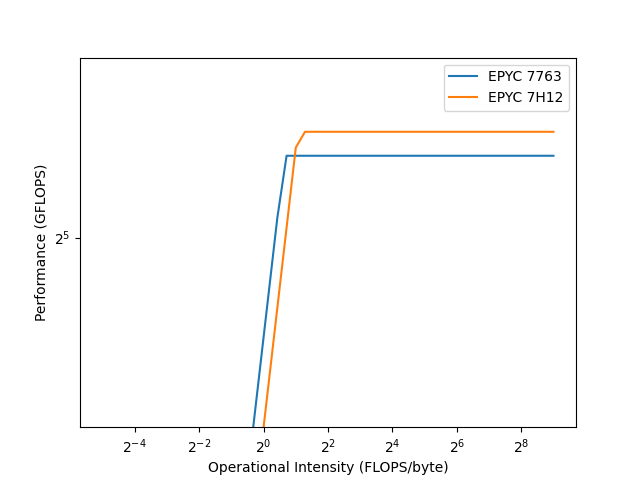
\includegraphics[width=\textwidth]{roofline_plot.png}
\caption{Roofline Model}
\label{fig:roofline}
\end{figure}

As we can see from the formula, the performance is limited by the bandwidth when $\pi < \beta \cdot I$ and by the peak performance when $\pi \geq \beta \cdot I$.
In the graph this can be seen visually. As long as the performance is still increasing we are limited by the bandwidth and once the performance plateaus we are limited by the peak performance.



\section{Auto-vectorization [10 points]}

1. Why is it important for data structures to be aligned? \\

Alligned data structures are important because the vectorization process requires that the data be contiguous in memory and alligned. 
Unalligned memory access can cause a performance penalty. 
If allignment is not specified, the compiler will be forced to generate runtime alignment optimization in order to be able to vectorize the code,
which will cause unecessary overhead or even prevent the vectorization.


2. What are some obstacles that can prevent automatic vectorization by the compiler? \\

- Function calls \\
- Data dependencies \\
- Data-dependent loop exit conditions \\
- Non-contiguous data \\

3. Is there a way to help the compiler to vectorize and how? \\

Yes, we can provide the compiler with extra information in the form of pragmas or compiler flags. \\

Some examples:
\begin{verbatim}
    #pragma vector align
\end{verbatim}
for example can assert that the data is alligned in memory which saves the compiler from having to generate runtime alignment optimization.
\begin{verbatim}
    #pragma ivdep
\end{verbatim}
Tells the compiler to ignore potential dependencies in the loop and vectorize it anyway. 
This can be helpful if the compiler is not able to detect that the loop is safe to vectorize but we insure that it is in some other part of our code.\\

4. Which loop optimizations are performed by the compiler to vectorize and pipeline loops?\\
Loop unrolling: The compiler will generate code that executes multiple iterations of the loop at once. 
This is done to increase the number of iterations that are executed in parallel. \\
Strip mining: The compiler will split the loop into smaller loops that are executed in parallel. 
This can increase the temporal and spacial locality of the data. \\

5. What can be done if automatic vectorization by the compiler fails or is sub-optimal?
First we can try to provide the compiler with more information to help it vectorize the code.
If it still fails we will have to manually vectorize the code. 
This can be done by using intrinsics or by using a library that provides vectorized operations.

\section{Matrix multiplication optimization [30 points]}

The first optimization we do is to use blocking to improve the temporal and spacial locality of the data.
Here we split the matrix into smaller blocks and multiply these blocks instead of the entire matrix.
This will increase the temporal and spacial locality of the data and reduce the number of cache misses.
\\
It is important to maximize the stride one access pattern to maximize the performance of the cache. 
This leads us to changing the order of the loops from the naive i,j,k to j,k,i. 
We then notice that in the last loop where we iterate over i we always multiply the same elements of the matrix B.
We can therefore load this element into memory only once before each iteration of the innermost loop and save a lot of memory accesses.
\\
In order to find the optimal blocksize we have to look at the cache sizes.
We can then use the formula $blocksize = \sqrt{\frac{{\text{{cache size}}}}{{3 \times \text{{sizeof(double)}}}}}$ as we have to fit 3 blocks into the cache at the same time.
Plugging the L1 cache size of 32KB into the formula we get a blocksize of 36 which is way to small to be efficient.
Using the L2 cache size of 512KB we get a blocksize of 146 which is a good starting point.
Through test we see that the performance difference between 100 and 150 is not very big. 
Anything above 150 will start to decrease the performance so we go with the theoretical optimal blocksize of 146.
\begin{figure}[H]
    \centering
    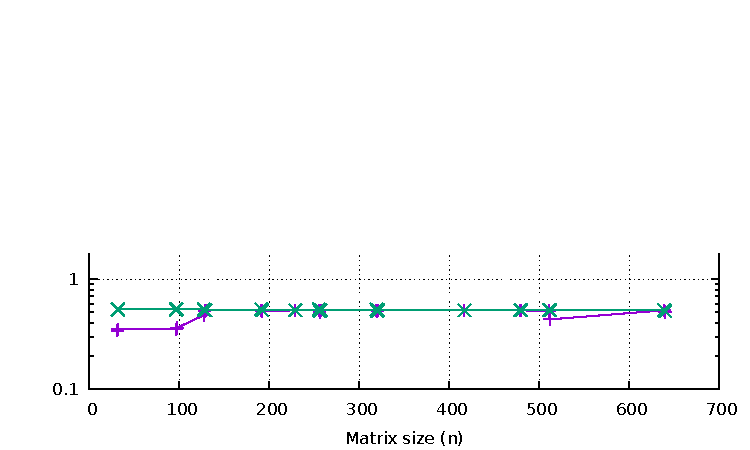
\includegraphics[width=0.7\linewidth]{timing_64.pdf}
    \caption{Block size 64}
    \label{fig:image1}
    
    \vspace{10pt}
    
    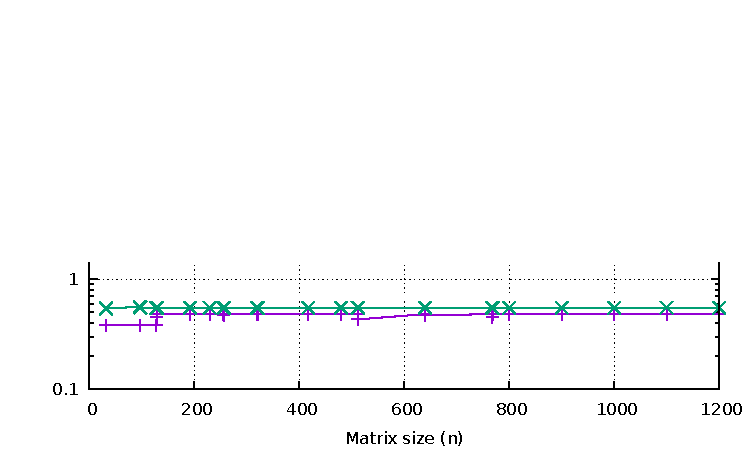
\includegraphics[width=0.7\linewidth]{timing_146.pdf}
    \caption{Block size 146}
    \label{fig:image2}
    
    \vspace{10pt}
    
    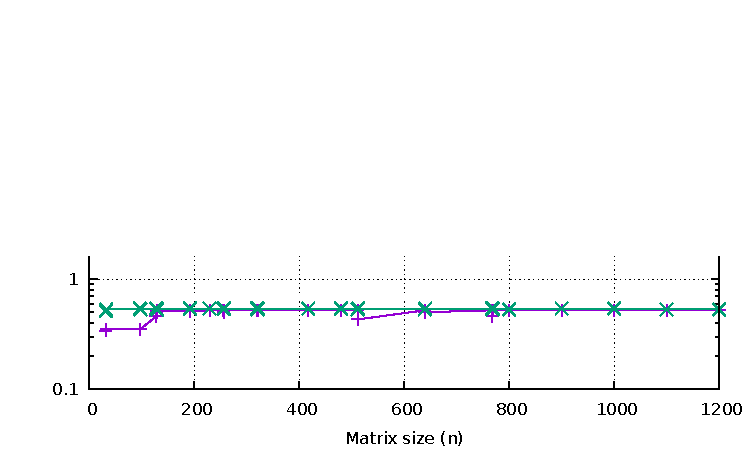
\includegraphics[width=0.7\linewidth]{timing_200.pdf}
    \caption{Block size 200}
    \label{fig:image3}
\end{figure}

The pragma vector aligned is used to assert that the data is alligned in memory which saves the compiler from having to generate runtime alignment optimization.
Another pragma that is used is the ivdep pragma which tells the compiler to ignore potential dependencies in the loop.
The same effect can be used by using the restrict keyword to tell the compiler that the pointers are not aliased. 
This combined with setting the optimization level to -O3 will allow the compiler to perform more aggressive optimizations.

\begin{figure}[h!]
    \centering
    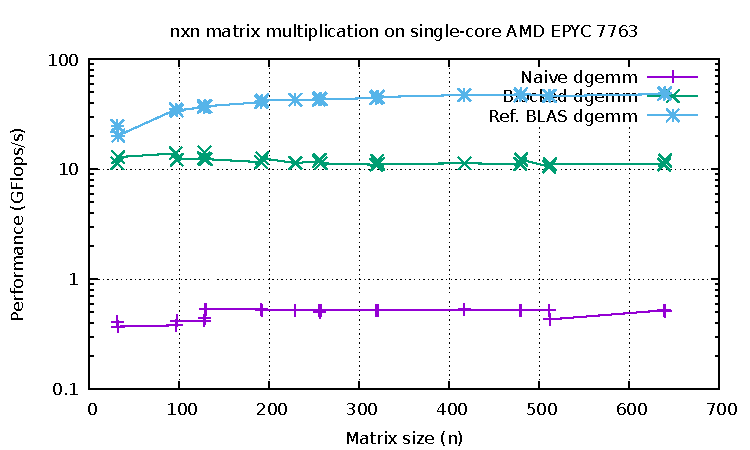
\includegraphics[width=0.7\linewidth]{timing_no_march.pdf}
    \caption{After the above optimizations}
    \label{fig:image}
\end{figure}

The final simple optimization we do is to use the -march=native flag in order to allow the compiler to generate code that is optimized for the specific architecture that we are running on.
This alone adds a significant performance improvement.

\begin{figure}[h!]
    \centering
    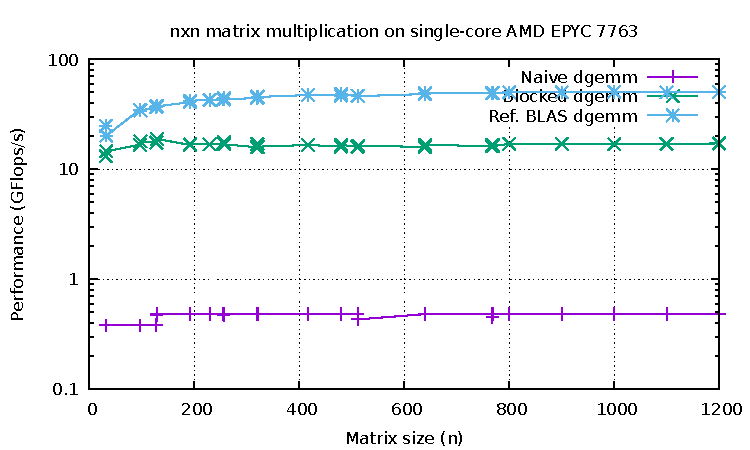
\includegraphics[width=0.7\linewidth]{timing_all.pdf}
    \caption{With architecture specific optimizations}
    \label{fig:image}
\end{figure}

After all these optimizations we can see a speedup from about 0.5 GFLOPS to 10 to 15 GFLOPS which is a significant improvement.
This is still slower than the performance of specialized libraries such as BLAS which reach speeds of 20 to 30 GFLOPS.


\end{document}
